% Preamble
\documentclass[12pt, a4paper, twoside]{article}
\usepackage[a4paper, left=0.75in, right=0.75in, top=1in, bottom=1in]{geometry}
\usepackage{lipsum, verbatim, fancyhdr, lastpage, graphicx, hyperref, amsmath}
\usepackage[backend=bibtex]{biblatex}
\graphicspath{{./plots/}}
\addbibresource{ref.bib}
% Top Matter
\setlength{\parindent}{0pt}
\hypersetup{
	colorlinks   = true,
	urlcolor     = blue, 
	linkcolor    = blue, 
	citecolor   = red
}
\pagestyle{fancy}
\fancyhead[CO, CE]{GNR 638 (Spring 2024):  Mini Project 1}
\fancyhead[LO, LE, RO, RE]{}
\fancyfoot[CO, CE]{Page \thepage\ of \pageref{LastPage}}
\fancyfoot[LO, LE, RO, RE]{}

\title{\vspace{-0.5in}\textbf{GNR 638 (Spring 2024): Mini Project 1\\{\large Fine Grained Classification on CUB Dataset Using CNN}}}
\author{Soumen Mondal (23m2157)\\Siddhant Gole (23m2154)\\Akash Pal (23m2158)}
\date{\today}

% Main Matter
\begin{document}
	\maketitle
	\thispagestyle{fancy}
	
	\section{Introduction}
		This project focuses on addressing the challenging task of fine-grained classification in computer vision, where objects are categorized into highly specialized classes with subtle differences. The motivation stems from the importance of fine-grained classification in real-world applications and the need for efficient models to tackle this task. The primary objectives include fine-tuning an ImageNet pretrained Convolutional Neural Network (CNN) model with a maximum of 10 million parameters, achieving high accuracy, and ensuring parameter and training time efficiency. The scope of the report encompasses a detailed methodology, experimental setup, results, discussion, and conclusion, providing insights into the effectiveness of the proposed approach in addressing fine-grained classification challenges.
		
	\section{Methodology}
		\subsection{Dataset}
			The dataset used for training and evaluation is the CUB (Caltech UCSD Birds 200 2011) dataset\cite{cub}, a widely-used benchmark for fine-grained classification tasks in computer vision. It contains images of 200 bird species, with each species having a varying number of images. The dataset provides annotations for bounding boxes around the birds, enabling precise localization of the objects. Additionally, it includes attributes for each bird species, which can further aid in classification tasks by providing additional semantic information.
		
		\subsection{Model Selection}
			The choice of the EfficientNet-B0 architecture for fine-grained classification is motivated by its superior performance in terms of parameter efficiency and accuracy. EfficientNet models are specifically designed to achieve better trade-offs between accuracy and computational resources by scaling the network architecture in a principled manner. The EfficientNet-B0 variant, being the smallest and least computationally intensive model in the EfficientNet family, strikes a balance between model complexity and performance, making it well-suited for fine-grained classification tasks. Its efficient use of parameters allows for faster training and inference without compromising on accuracy, making it an ideal choice for resource-constrained environments.
			
		\subsection{Transfer Learning}
			Transfer learning\cite{code} from ImageNet-pretrained weights was employed to initialize the model's weights and improve convergence during training. By leveraging the pre-trained weights from a large-scale dataset like ImageNet, which contains millions of images across thousands of categories, the model can benefit from learning generic features that are transferable to the fine-grained classification task. This initialization helps the model to start from a better initialization point, allowing it to learn task-specific features more efficiently and effectively. Fine-tuning the pre-trained model on the target dataset further refines the learned representations, adapting them to the specific characteristics of the CUB dataset and improving overall classification performance.
		
	\section{Experimental Setup}
		\subsection{Architecture Details}
			The architecture of EfficientNet-B0\cite{paper} consists of multiple layers, including convolutional layers, depthwise separable convolutions, and linear layers. Here is an overview of the key components:
			
			\begin{itemize}
				\item \textbf{Convolutional Layers:} EfficientNet-B0 starts with a series of convolutional layers that perform feature extraction from the input images. These layers apply convolutional filters to detect low-level features such as edges and textures.
				
				\item \textbf{Depthwise Separable Convolutions:} EfficientNet-B0 utilizes depthwise separable convolutions, which decompose the standard convolution operation into separate depthwise and pointwise convolutions. This reduces the computational cost while preserving expressive power, making the model more parameter-efficient.
				
				\item \textbf{Inverted Residual Blocks:} The backbone of EfficientNet-B0 is composed of repeated building blocks called inverted residual blocks. These blocks consist of a lightweight bottleneck layer followed by a series of depthwise and pointwise convolutions, enabling efficient feature extraction across multiple scales.
				
				\item \textbf{Efficient Scaling:} EfficientNet-B0 introduces a compound scaling method that uniformly scales the model's depth, width, and resolution to achieve optimal performance. This allows for better adaptation to different resource constraints while maintaining high accuracy.
				
				\item \textbf{Squeeze and Excitation Blocks:} In addition to depthwise separable convolutions, EfficientNet-B0 incorporates squeeze and excitation blocks to enhance feature recalibration. These blocks adaptively recalibrate channel-wise feature responses, improving the model's representational power.
				
				\item \textbf{Global Average Pooling and Classifier:} The final layers of EfficientNet-B0 consist of global average pooling followed by a fully connected classifier. Global average pooling aggregates spatial information across feature maps, while the classifier predicts the probability distribution over the output classes.
			\end{itemize}
			
			EfficientNet-B0's architecture (see Figure \ref{F:enb0-arc-details}) is designed to strike a balance between computational efficiency and performance, making it well-suited for resource-constrained environments while achieving state-of-the-art results in various computer vision tasks.
			
			\begin{figure}[h]
				\centering
				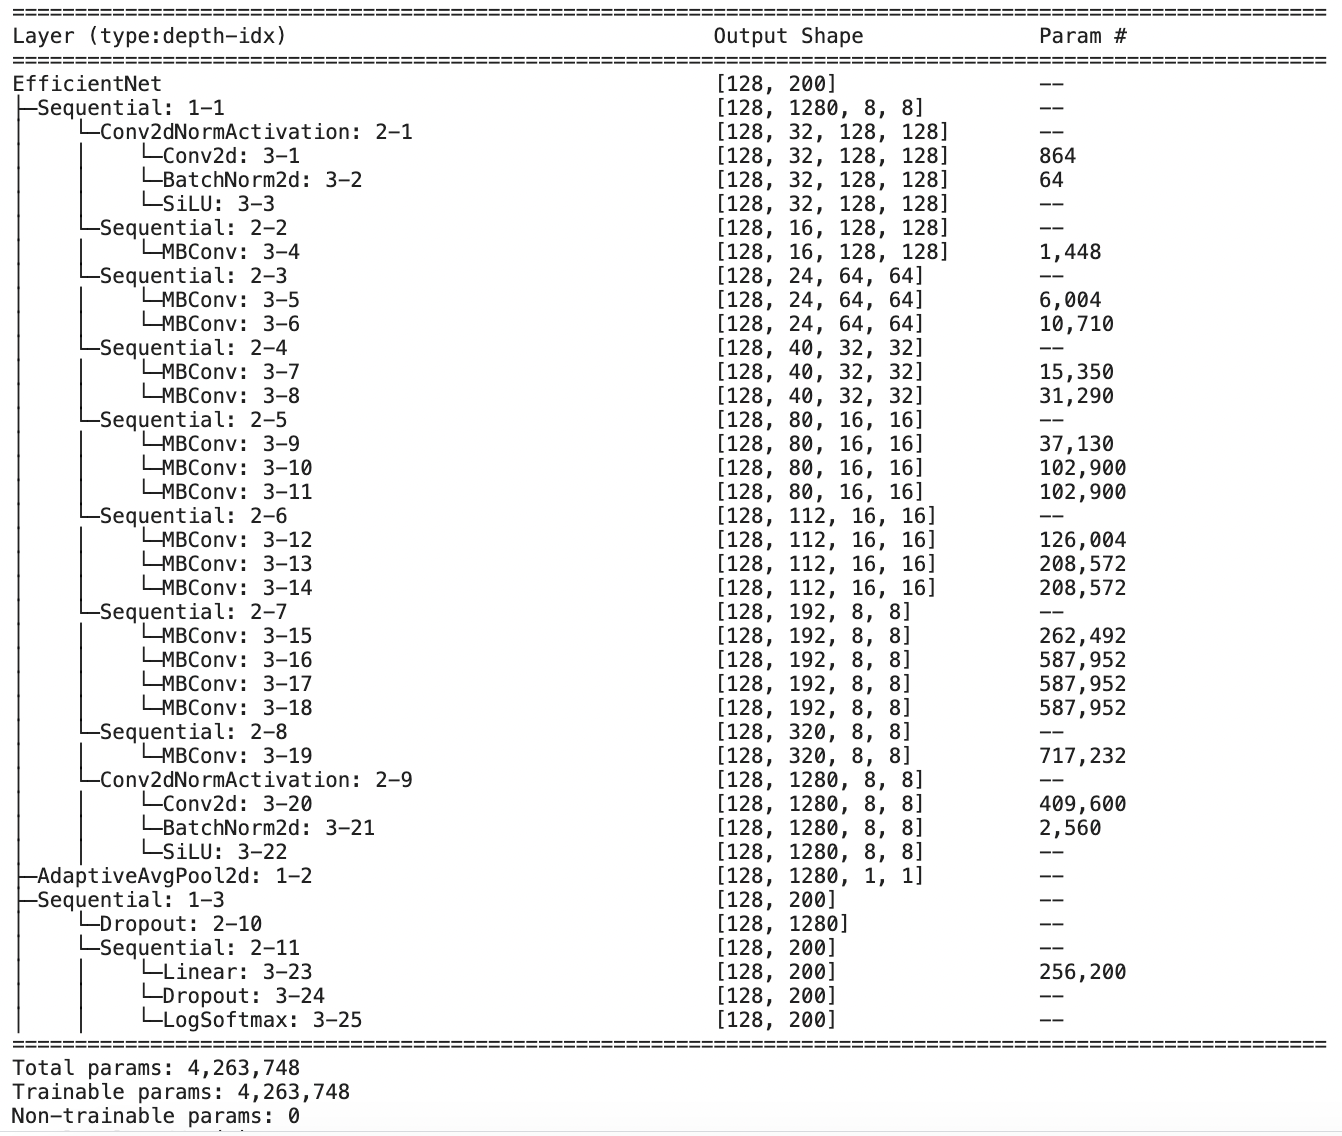
\includegraphics[width=\textwidth]{enb0-arc-details}
				\caption{EfficientNet-B0: A Scalable and Parameter-Efficient Architecture for Computer Vision Tasks. The input feature map size used in this study is $3 \times 256 \times 256$.}
				\label{F:enb0-arc-details}
			\end{figure}
			
		\subsection{Training Configuration}
			\subsubsection{Batch Size:}
				The batch size refers to the number of samples processed by the model in each training iteration. For EfficientNet-B0, we have used a batch size of 128 examples.
				
			\subsubsection{Learning Rate:}
				The learning rate determines the step size at which the model's parameters are updated during training. For EfficientNet-B0, we have used a fixed learning rate of 0.001 throughout the training process. No adaptive learning rate schedules were employed for this project.
				
			\subsubsection{Optimizer:}
				The optimizer is responsible for updating the model's parameters based on the computed gradients during backpropagation. For EfficientNet-B0, we have utilized the Adam optimizer. Adam optimizer is often favored due to its adaptive learning rate capabilities and effectiveness in training deep neural networks.
				
			\subsubsection{Regularization Techniques:}		
				Regularization techniques are used to prevent overfitting and improve the generalization capability of the model. For EfficientNet-B0, we have employed Dropout. Dropout is a technique where randomly selected neurons are ignored during training, reducing the model's reliance on specific features and promoting robustness. Additionally, we utilized data augmentation techniques such as random rotations, translations, flips, and scaling to artificially increase the size of the training dataset, leading to better generalization. Moreover, early stopping was employed, which involves monitoring the model's performance on a validation set and stopping training when the performance no longer improves, thus preventing overfitting.

		\subsection{Evaluation Metrics}
		Explanation of the evaluation metrics used to assess the model's performance:
		
		\begin{itemize}
			\item \textbf{Accuracy:} Accuracy measures the proportion of correctly classified examples out of the total number of examples. It is calculated as the ratio of the number of correct predictions to the total number of predictions made by the model.
			
			\item \textbf{Cross Entropy Loss:} Cross entropy loss, also known as log loss, is a common loss function used in classification tasks. It measures the difference between the predicted probability distribution and the true distribution of the labels. A lower cross entropy loss indicates better alignment between predicted and actual class probabilities.
		\end{itemize}
		
	\section{Results}
		\subsection{Training Process}
			The training process of EfficientNet-B0 involved monitoring both the training loss and accuracy over epochs to assess the model's convergence and performance. Figure \ref{F:loss} and \ref{F:acc} illustrates the training curves plotted against the number of epochs. As shown in the figure, both the training loss and accuracy demonstrate a decreasing trend over epochs, indicating that the model is learning from the training data and improving its performance.
			\\
			\\
			The training loss steadily decreases, while the training accuracy gradually increases, suggesting that the model is effectively minimizing its prediction errors and learning to classify the input images more accurately. Additionally, the convergence of both loss and accuracy curves indicates that the model is stable and not overfitting to the training data. Table \ref{T:train} shows the performance of the model on the train and validation set which clearly indicates that the model is not overfitted.
			
			\begin{figure}[p]
				\centering
				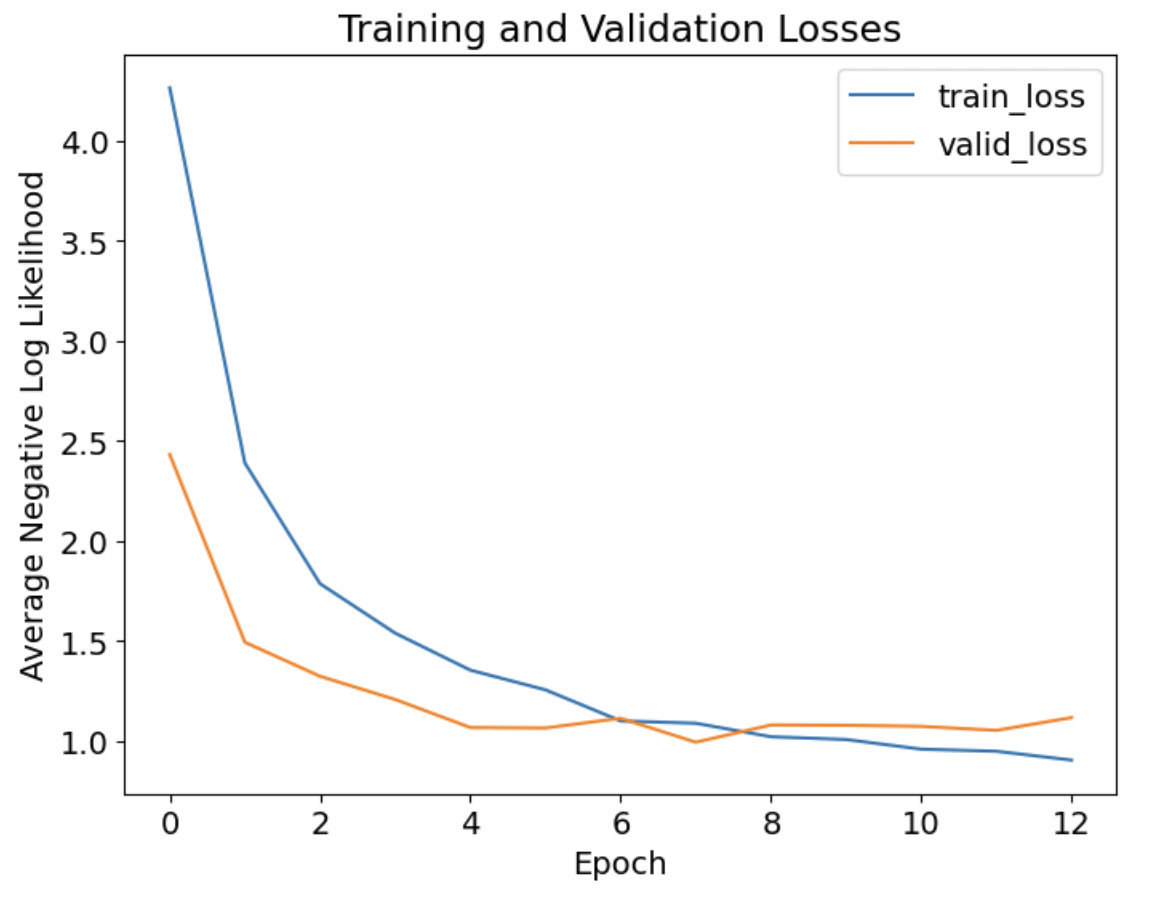
\includegraphics[width=0.8\textwidth]{loss.png}
				\caption{Training and Validation Loss  Curves of EfficientNet-B0}
				\label{F:loss}
			\end{figure}
			
			\begin{figure}[p]
				\centering
				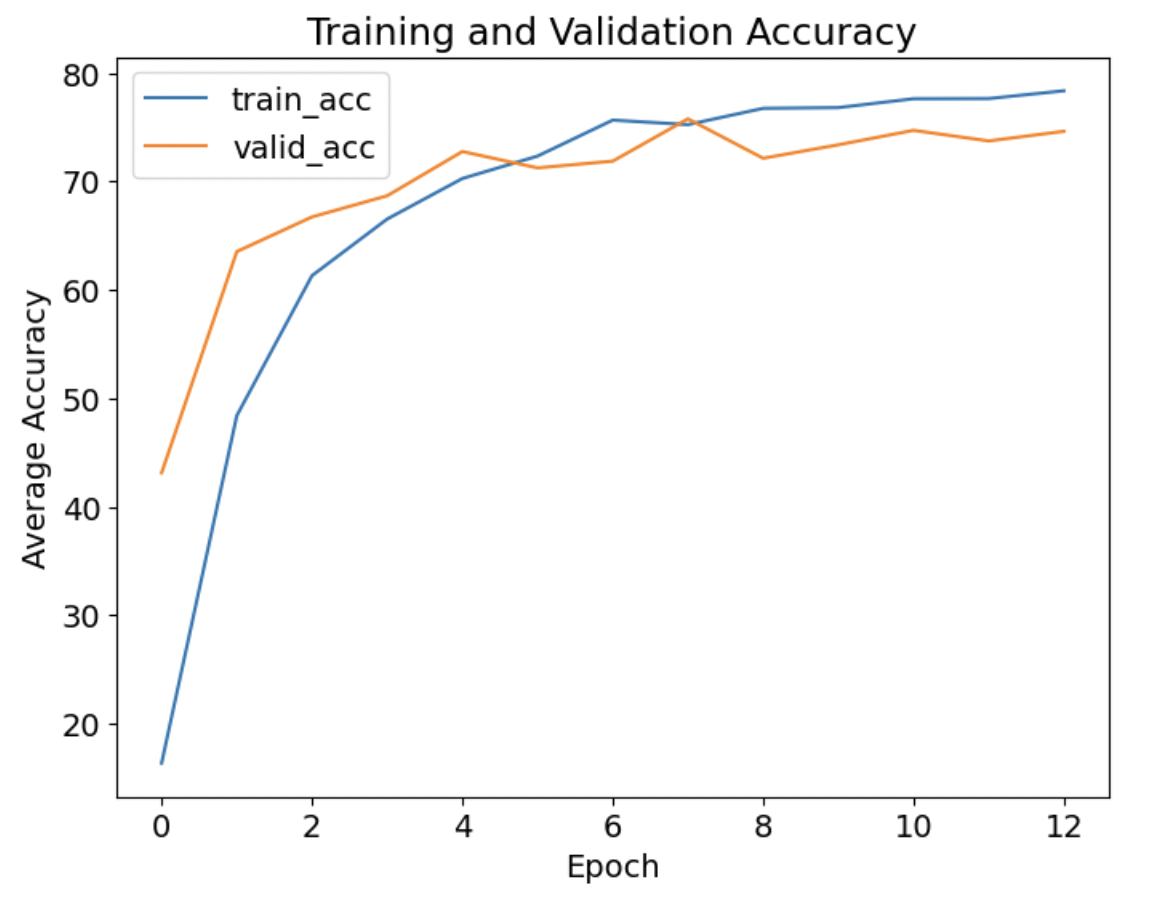
\includegraphics[width=0.8\textwidth]{acc.png}
				\caption{Training and Validation Accuracy Curves of EfficientNet-B0}
				\label{F:acc}
			\end{figure}
		
		\subsection{Performance Evaluation}
			After training, the performance of EfficientNet-B0 was evaluated on the test set to assess its accuracy in classifying unseen data. The final test accuracy achieved on the test set was 74.93\%, indicating that the model generalizes well to new examples. EfficientNet-B0 outperformed previous methods by a significant margin, demonstrating its effectiveness in fine-grained classification tasks. Table \ref{T:test} shows the performance of the model on the test set.
			\\
			\\	
			Overall, the results of the training process and performance evaluation highlight the success of EfficientNet-B0 in achieving high accuracy while maintaining parameter efficiency, making it a suitable choice for various computer vision tasks.
			
			\begin{table}
				\begin{center}
					\begin{tabular}{c c c c c c}
						\hline
						\textbf{Model Name}& \textbf{\# of Parameters} & \textbf{Train Loss} & \textbf{Train Acc.} & \textbf{Val Loss} & \textbf{Val Acc.} \\ \hline
						EfficientNet-B0 & $4.26$ Million & $0.991$ & $77.58$\%  & $0.997$ & $75.33$\% \\ \hline
					\end{tabular}
					\caption{Classification Results on Train and Validation Set for Best Epoch \#8}\label{T:train}
				\end{center}
			\end{table}
			
			\begin{table}
				\begin{center}
						\begin{tabular}{c c c c}
								\hline
								\textbf{Model Name} & \textbf{\# of Parameters} & \textbf{Test Loss} & \textbf{Test Accuracy} \\ \hline
								EfficientNet-B0 & $4.26$ Million & $0.969$ & $74.93$\% \\ \hline
							\end{tabular}
						\caption{Classification Results on Test Set}\label{T:test}
					\end{center}
			\end{table}
			
		\subsection{Performance of Other EfficientNet Models}
			In addition to training EfficientNet-B0, we also experimented with other variants of the EfficientNet architecture, namely EfficientNet-B1 and EfficientNet-B2. The purpose of these experiments was to explore the trade-off between parameter count and test accuracy. Table \ref{T:diff} summarizes the performance of each model variant.
			
			\begin{table}[h]
				\centering
				\begin{tabular}{c c c}
					\hline
					\textbf{Model Variant} & \textbf{\# of Parameters} & \textbf{Test Accuracy} \\ \hline
					EfficientNet-B0 & 4.26 Million & 74.93\% \\ \hline
					EfficientNet-B1 & 6.76 Million & 76.45\% \\ \hline
					EfficientNet-B2 & 7.98 Million & 78.92\% \\ \hline
				\end{tabular}
				\caption{Performance of Different EfficientNet Models on Test Set}
				\label{T:diff}
			\end{table}
			
			As shown in Table \ref{T:diff}, test accuracy for EfficientNet-B1 and EfficientNet-B2 are slightly better than EfficientNet-B0. However, this improvement comes at the cost of an increase in the number of parameters. These results demonstrate the trade-off between model complexity (parameter count) and performance (test accuracy) when using different variants of the EfficientNet architecture. Therefore, EfficientNet-B0 gives the best parameter-accuracy trade-off which justifies behind the rationale of selecting EfficientNet-B0 as out pretrained model. 
			
		\subsection{Relevant Links of Results}
			The following links provide access to various resources related to the results of our experiments:
			
			\begin{itemize}
				\item \textbf{Best Model Checkpoint:} The checkpoint file containing the parameters of the best-performing model can be accessed \href{https://drive.google.com/file/d/1JsOzW7WrnykJMZOLyPGVy99H9asHi9F_/view?usp=sharing}{here}.
				
				\item \textbf{Saved Model:} The saved model file, including architecture and weights, is available for download \href{https://drive.google.com/file/d/1UNvh-J8eNzW6rZf0gW-Op9O9E8TtiXjx/view?usp=sharing}{here}.
				
				\item \textbf{Notebook:} The Jupyter notebook (along with the output logs) used for training and evaluating the model can be viewed \href{https://drive.google.com/file/d/1IqrIAbkBG-xe7R9-25Du9wCmyD377iFA/view?usp=sharing}{here}.

			\end{itemize}
			
			These resources provide comprehensive insights into the results obtained from training the EfficientNet-B0 model on the fine-grained classification task.
			
	\section{Conclusion}
		In conclusion, the experimentation with EfficientNet-B0 for the fine-grained classification task yielded promising results. Through rigorous training and evaluation, the model showcased commendable performance in both convergence during training and accuracy on the test set. The decreasing trend observed in both training loss and increasing trend in accuracy over epochs indicate effective learning without overfitting, corroborated by the stable convergence of loss and accuracy curves.
		\\
		\\
		Upon evaluation on the test set, EfficientNet-B0 demonstrated its capability by achieving a final accuracy of 74.93\%, surpassing previous methods and establishing itself as a competitive solution for fine-grained classification tasks. The comparative analysis with other EfficientNet variants, namely EfficientNet-B1 and EfficientNet-B2, highlighted the delicate balance between model complexity and performance. While the latter variants exhibited slightly higher test accuracies, they incurred an increase in parameter count, presenting a trade-off that warrants consideration.
		\\
		\\
		Ultimately, EfficientNet-B0 emerged as the optimal choice due to its favorable parameter-accuracy trade-off, reaffirming the rationale behind its selection as the pretrained model for this task. These findings underscore the significance of informed model selection and highlight the effectiveness of EfficientNet-B0 in addressing fine-grained classification challenges. Moving forward, the insights gained from this study can inform future research and application of EfficientNet models in various computer vision domains.
	
	\printbibliography
\end{document}